
%% bare_jrnl_compsoc.tex
%% V1.4b
%% 2015/08/26
%% by Michael Shell
%% See:
%% http://www.michaelshell.org/
%% for current contact information.
%%
%% This is a skeleton file demonstrating the use of IEEEtran.cls
%% (requires IEEEtran.cls version 1.8b or later) with an IEEE
%% Computer Society journal paper.
%%
%% Support sites:
%% http://www.michaelshell.org/tex/ieeetran/
%% http://www.ctan.org/pkg/ieeetran
%% and
%% http://www.ieee.org/

%%*************************************************************************
%% Legal Notice:
%% This code is offered as-is without any warranty either expressed or
%% implied; without even the implied warranty of MERCHANTABILITY or
%% FITNESS FOR A PARTICULAR PURPOSE! 
%% User assumes all risk.
%% In no event shall the IEEE or any contributor to this code be liable for
%% any damages or losses, including, but not limited to, incidental,
%% consequential, or any other damages, resulting from the use or misuse
%% of any information contained here.
%%
%% All comments are the opinions of their respective authors and are not
%% necessarily endorsed by the IEEE.
%%
%% This work is distributed under the LaTeX Project Public License (LPPL)
%% ( http://www.latex-project.org/ ) version 1.3, and may be freely used,
%% distributed and modified. A copy of the LPPL, version 1.3, is included
%% in the base LaTeX documentation of all distributions of LaTeX released
%% 2003/12/01 or later.
%% Retain all contribution notices and credits.
%% ** Modified files should be clearly indicated as such, including  **
%% ** renaming them and changing author support contact information. **
%%*************************************************************************


% *** Authors should verify (and, if needed, correct) their LaTeX system  ***
% *** with the testflow diagnostic prior to trusting their LaTeX platform ***
% *** with production work. The IEEE's font choices and paper sizes can   ***
% *** trigger bugs that do not appear when using other class files.       ***                          ***
% The testflow support page is at:
% http://www.michaelshell.org/tex/testflow/


\documentclass[10pt,journal,compsoc]{IEEEtran}
%
% If IEEEtran.cls has not been installed into the LaTeX system files,
% manually specify the path to it like:
% \documentclass[10pt,journal,compsoc]{../sty/IEEEtran}





% Some very useful LaTeX packages include:
% (uncomment the ones you want to load)


% *** MISC UTILITY PACKAGES ***
%
%\usepackage{ifpdf}
% Heiko Oberdiek's ifpdf.sty is very useful if you need conditional
% compilation based on whether the output is pdf or dvi.
% usage:
% \ifpdf
%   % pdf code
% \else
%   % dvi code
% \fi
% The latest version of ifpdf.sty can be obtained from:
% http://www.ctan.org/pkg/ifpdf
% Also, note that IEEEtran.cls V1.7 and later provides a builtin
% \ifCLASSINFOpdf conditional that works the same way.
% When switching from latex to pdflatex and vice-versa, the compiler may
% have to be run twice to clear warning/error messages.






% *** CITATION PACKAGES ***
%
\ifCLASSOPTIONcompsoc
  % IEEE Computer Society needs nocompress option
  % requires cite.sty v4.0 or later (November 2003)
  \usepackage[nocompress]{cite}
\else
  % normal IEEE
  \usepackage{cite}
\fi
% cite.sty was written by Donald Arseneau
% V1.6 and later of IEEEtran pre-defines the format of the cite.sty package
% \cite{} output to follow that of the IEEE. Loading the cite package will
% result in citation numbers being automatically sorted and properly
% "compressed/ranged". e.g., [1], [9], [2], [7], [5], [6] without using
% cite.sty will become [1], [2], [5]--[7], [9] using cite.sty. cite.sty's
% \cite will automatically add leading space, if needed. Use cite.sty's
% noadjust option (cite.sty V3.8 and later) if you want to turn this off
% such as if a citation ever needs to be enclosed in parenthesis.
% cite.sty is already installed on most LaTeX systems. Be sure and use
% version 5.0 (2009-03-20) and later if using hyperref.sty.
% The latest version can be obtained at:
% http://www.ctan.org/pkg/cite
% The documentation is contained in the cite.sty file itself.
%
% Note that some packages require special options to format as the Computer
% Society requires. In particular, Computer Society  papers do not use
% compressed citation ranges as is done in typical IEEE papers
% (e.g., [1]-[4]). Instead, they list every citation separately in order
% (e.g., [1], [2], [3], [4]). To get the latter we need to load the cite
% package with the nocompress option which is supported by cite.sty v4.0
% and later. Note also the use of a CLASSOPTION conditional provided by
% IEEEtran.cls V1.7 and later.





% *** GRAPHICS RELATED PACKAGES ***
%
\ifCLASSINFOpdf
  \usepackage[pdftex]{graphicx}
  \usepackage{subfigure}
  % declare the path(s) where your graphic files are
  % \graphicspath{{../pdf/}{../jpeg/}}
  % and their extensions so you won't have to specify these with
  % every instance of \includegraphics
  % \DeclareGraphicsExtensions{.pdf,.jpeg,.png}
\else
  % or other class option (dvipsone, dvipdf, if not using dvips). graphicx
  % will default to the driver specified in the system graphics.cfg if no
  % driver is specified.
  % \usepackage[dvips]{graphicx}
  % declare the path(s) where your graphic files are
  % \graphicspath{{../eps/}}
  % and their extensions so you won't have to specify these with
  % every instance of \includegraphics
  % \DeclareGraphicsExtensions{.eps}
\fi
% graphicx was written by David Carlisle and Sebastian Rahtz. It is
% required if you want graphics, photos, etc. graphicx.sty is already
% installed on most LaTeX systems. The latest version and documentation
% can be obtained at: 
% http://www.ctan.org/pkg/graphicx
% Another good source of documentation is "Using Imported Graphics in
% LaTeX2e" by Keith Reckdahl which can be found at:
% http://www.ctan.org/pkg/epslatex
%
% latex, and pdflatex in dvi mode, support graphics in encapsulated
% postscript (.eps) format. pdflatex in pdf mode supports graphics
% in .pdf, .jpeg, .png and .mps (metapost) formats. Users should ensure
% that all non-photo figures use a vector format (.eps, .pdf, .mps) and
% not a bitmapped formats (.jpeg, .png). The IEEE frowns on bitmapped formats
% which can result in "jaggedy"/blurry rendering of lines and letters as
% well as large increases in file sizes.
%
% You can find documentation about the pdfTeX application at:
% http://www.tug.org/applications/pdftex






% *** MATH PACKAGES ***
%
\usepackage{listings}
\usepackage{amsmath}
\usepackage{amsthm}
% A popular package from the American Mathematical Society that provides
% many useful and powerful commands for dealing with mathematics.
%
% Note that the amsmath package sets \interdisplaylinepenalty to 10000
% thus preventing page breaks from occurring within multiline equations. Use:
%\interdisplaylinepenalty=2500
% after loading amsmath to restore such page breaks as IEEEtran.cls normally
% does. amsmath.sty is already installed on most LaTeX systems. The latest
% version and documentation can be obtained at:
% http://www.ctan.org/pkg/amsmath





% *** SPECIALIZED LIST PACKAGES ***
%
\usepackage{algorithm}
\usepackage{algorithmic}
% algorithmic.sty was written by Peter Williams and Rogerio Brito.
% This package provides an algorithmic environment fo describing algorithms.
% You can use the algorithmic environment in-text or within a figure
% environment to provide for a floating algorithm. Do NOT use the algorithm
% floating environment provided by algorithm.sty (by the same authors) or
% algorithm2e.sty (by Christophe Fiorio) as the IEEE does not use dedicated
% algorithm float types and packages that provide these will not provide
% correct IEEE style captions. The latest version and documentation of
% algorithmic.sty can be obtained at:
% http://www.ctan.org/pkg/algorithms
% Also of interest may be the (relatively newer and more customizable)
% algorithmicx.sty package by Szasz Janos:
% http://www.ctan.org/pkg/algorithmicx




% *** ALIGNMENT PACKAGES ***
%
%\usepackage{array}
% Frank Mittelbach's and David Carlisle's array.sty patches and improves
% the standard LaTeX2e array and tabular environments to provide better
% appearance and additional user controls. As the default LaTeX2e table
% generation code is lacking to the point of almost being broken with
% respect to the quality of the end results, all users are strongly
% advised to use an enhanced (at the very least that provided by array.sty)
% set of table tools. array.sty is already installed on most systems. The
% latest version and documentation can be obtained at:
% http://www.ctan.org/pkg/array


% IEEEtran contains the IEEEeqnarray family of commands that can be used to
% generate multiline equations as well as matrices, tables, etc., of high
% quality.




% *** SUBFIGURE PACKAGES ***
%\ifCLASSOPTIONcompsoc
%  \usepackage[caption=false,font=footnotesize,labelfont=sf,textfont=sf]{subfig}
%\else
%  \usepackage[caption=false,font=footnotesize]{subfig}
%\fi
% subfig.sty, written by Steven Douglas Cochran, is the modern replacement
% for subfigure.sty, the latter of which is no longer maintained and is
% incompatible with some LaTeX packages including fixltx2e. However,
% subfig.sty requires and automatically loads Axel Sommerfeldt's caption.sty
% which will override IEEEtran.cls' handling of captions and this will result
% in non-IEEE style figure/table captions. To prevent this problem, be sure
% and invoke subfig.sty's "caption=false" package option (available since
% subfig.sty version 1.3, 2005/06/28) as this is will preserve IEEEtran.cls
% handling of captions.
% Note that the Computer Society format requires a sans serif font rather
% than the serif font used in traditional IEEE formatting and thus the need
% to invoke different subfig.sty package options depending on whether
% compsoc mode has been enabled.
%
% The latest version and documentation of subfig.sty can be obtained at:
% http://www.ctan.org/pkg/subfig




% *** FLOAT PACKAGES ***
%
%\usepackage{fixltx2e}
% fixltx2e, the successor to the earlier fix2col.sty, was written by
% Frank Mittelbach and David Carlisle. This package corrects a few problems
% in the LaTeX2e kernel, the most notable of which is that in current
% LaTeX2e releases, the ordering of single and double column floats is not
% guaranteed to be preserved. Thus, an unpatched LaTeX2e can allow a
% single column figure to be placed prior to an earlier double column
% figure.
% Be aware that LaTeX2e kernels dated 2015 and later have fixltx2e.sty's
% corrections already built into the system in which case a warning will
% be issued if an attempt is made to load fixltx2e.sty as it is no longer
% needed.
% The latest version and documentation can be found at:
% http://www.ctan.org/pkg/fixltx2e


%\usepackage{stfloats}
% stfloats.sty was written by Sigitas Tolusis. This package gives LaTeX2e
% the ability to do double column floats at the bottom of the page as well
% as the top. (e.g., "\begin{figure*}[!b]" is not normally possible in
% LaTeX2e). It also provides a command:
%\fnbelowfloat
% to enable the placement of footnotes below bottom floats (the standard
% LaTeX2e kernel puts them above bottom floats). This is an invasive package
% which rewrites many portions of the LaTeX2e float routines. It may not work
% with other packages that modify the LaTeX2e float routines. The latest
% version and documentation can be obtained at:
% http://www.ctan.org/pkg/stfloats
% Do not use the stfloats baselinefloat ability as the IEEE does not allow
% \baselineskip to stretch. Authors submitting work to the IEEE should note
% that the IEEE rarely uses double column equations and that authors should try
% to avoid such use. Do not be tempted to use the cuted.sty or midfloat.sty
% packages (also by Sigitas Tolusis) as the IEEE does not format its papers in
% such ways.
% Do not attempt to use stfloats with fixltx2e as they are incompatible.
% Instead, use Morten Hogholm'a dblfloatfix which combines the features
% of both fixltx2e and stfloats:
%
% \usepackage{dblfloatfix}
% The latest version can be found at:
% http://www.ctan.org/pkg/dblfloatfix




%\ifCLASSOPTIONcaptionsoff
%  \usepackage[nomarkers]{endfloat}
% \let\MYoriglatexcaption\caption
% \renewcommand{\caption}[2][\relax]{\MYoriglatexcaption[#2]{#2}}
%\fi
% endfloat.sty was written by James Darrell McCauley, Jeff Goldberg and 
% Axel Sommerfeldt. This package may be useful when used in conjunction with 
% IEEEtran.cls'  captionsoff option. Some IEEE journals/societies require that
% submissions have lists of figures/tables at the end of the paper and that
% figures/tables without any captions are placed on a page by themselves at
% the end of the document. If needed, the draftcls IEEEtran class option or
% \CLASSINPUTbaselinestretch interface can be used to increase the line
% spacing as well. Be sure and use the nomarkers option of endfloat to
% prevent endfloat from "marking" where the figures would have been placed
% in the text. The two hack lines of code above are a slight modification of
% that suggested by in the endfloat docs (section 8.4.1) to ensure that
% the full captions always appear in the list of figures/tables - even if
% the user used the short optional argument of \caption[]{}.
% IEEE papers do not typically make use of \caption[]'s optional argument,
% so this should not be an issue. A similar trick can be used to disable
% captions of packages such as subfig.sty that lack options to turn off
% the subcaptions:
% For subfig.sty:
% \let\MYorigsubfloat\subfloat
% \renewcommand{\subfloat}[2][\relax]{\MYorigsubfloat[]{#2}}
% However, the above trick will not work if both optional arguments of
% the \subfloat command are used. Furthermore, there needs to be a
% description of each subfigure *somewhere* and endfloat does not add
% subfigure captions to its list of figures. Thus, the best approach is to
% avoid the use of subfigure captions (many IEEE journals avoid them anyway)
% and instead reference/explain all the subfigures within the main caption.
% The latest version of endfloat.sty and its documentation can obtained at:
% http://www.ctan.org/pkg/endfloat
%
% The IEEEtran \ifCLASSOPTIONcaptionsoff conditional can also be used
% later in the document, say, to conditionally put the References on a 
% page by themselves.




% *** PDF, URL AND HYPERLINK PACKAGES ***
%
%\usepackage{url}
% url.sty was written by Donald Arseneau. It provides better support for
% handling and breaking URLs. url.sty is already installed on most LaTeX
% systems. The latest version and documentation can be obtained at:
% http://www.ctan.org/pkg/url
% Basically, \url{my_url_here}.

% Extra Packages
\usepackage{booktabs}
\usepackage{url}

% Extra Commands
\DeclareMathOperator*{\argmin}{arg\,min}


% *** Do not adjust lengths that control margins, column widths, etc. ***
% *** Do not use packages that alter fonts (such as pslatex).         ***
% There should be no need to do such things with IEEEtran.cls V1.6 and later.
% (Unless specifically asked to do so by the journal or conference you plan
% to submit to, of course. )


% correct bad hyphenation here
\hyphenation{op-tical net-works semi-conduc-tor}


\begin{document}
%
% paper title
% Titles are generally capitalized except for words such as a, an, and, as,
% at, but, by, for, in, nor, of, on, or, the, to and up, which are usually
% not capitalized unless they are the first or last word of the title.
% Linebreaks \\ can be used within to get better formatting as desired.
% Do not put math or special symbols in the title.
\title{Introduction to Web Search and Mining\\Option A - Project Report}
%
%
% author names and IEEE memberships
% note positions of commas and nonbreaking spaces ( ~ ) LaTeX will not break
% a structure at a ~ so this keeps an author's name from being broken across
% two lines.
% use \thanks{} to gain access to the first footnote area
% a separate \thanks must be used for each paragraph as LaTeX2e's \thanks
% was not built to handle multiple paragraphs
%
%
%\IEEEcompsocitemizethanks is a special \thanks that produces the bulleted
% lists the Computer Society journals use for "first footnote" author
% affiliations. Use \IEEEcompsocthanksitem which works much like \item
% for each affiliation group. When not in compsoc mode,
% \IEEEcompsocitemizethanks becomes like \thanks and
% \IEEEcompsocthanksitem becomes a line break with idention. This
% facilitates dual compilation, although admittedly the differences in the
% desired content of \author between the different types of papers makes a
% one-size-fits-all approach a daunting prospect. For instance, compsoc 
% journal papers have the author affiliations above the "Manuscript
% received ..."  text while in non-compsoc journals this is reversed. Sigh.

% \author{Ruoyu~Deng~118033910030, Xutong~Lu~118033910116, Fuming~Zhang~118033910025, and~Wencai~Zhong~118033910101
\author{Ruoyu~Deng, Xutong~Lu, Fuming~Zhang, and~Wencai~Zhong \\
118033910030, 118033910116, 118033910025, and~118033910101
\IEEEcompsocitemizethanks{\IEEEcompsocthanksitem Project Link: https://github.com/AlexChang/WSM-SOSearch
\IEEEcompsocthanksitem Raw Data Link: https://pan.baidu.com/s/16\_C4dFrXuUfPwuurDWZFIA Extraction Code: ne6l 
\IEEEcompsocthanksitem Database Link: https://pan.baidu.com/s/1lCxzOB9GWIRqG1L4Zf8eYg Extraction Code: qgao
\IEEEcompsocthanksitem Website Demo Link: http://202.120.38.54:8000, http://202.120.38.54:8001
\IEEEcompsocthanksitem E-mails: 767423930@qq.com, zhangfuming-alex@sjtu.edu.cn}}

% note the % following the last \IEEEmembership and also \thanks - 
% these prevent an unwanted space from occurring between the last author name
% and the end of the author line. i.e., if you had this:
% 
% \author{....lastname \thanks{...} \thanks{...} }
%                     ^------------^------------^----Do not want these spaces!
%
% a space would be appended to the last name and could cause every name on that
% line to be shifted left slightly. This is one of those "LaTeX things". For
% instance, "\textbf{A} \textbf{B}" will typeset as "A B" not "AB". To get
% "AB" then you have to do: "\textbf{A}\textbf{B}"
% \thanks is no different in this regard, so shield the last } of each \thanks
% that ends a line with a % and do not let a space in before the next \thanks.
% Spaces after \IEEEmembership other than the last one are OK (and needed) as
% you are supposed to have spaces between the names. For what it is worth,
% this is a minor point as most people would not even notice if the said evil
% space somehow managed to creep in.



% The paper headers
%\markboth{Journal of \LaTeX\ Class Files,~Vol.~14, No.~8, August~2015}%
%{Shell \MakeLowercase{\textit{et al.}}: Bare Demo of IEEEtran.cls for Computer Society Journals}
% The only time the second header will appear is for the odd numbered pages
% after the title page when using the twoside option.
% 
% *** Note that you probably will NOT want to include the author's ***
% *** name in the headers of peer review papers.                   ***
% You can use \ifCLASSOPTIONpeerreview for conditional compilation here if
% you desire.



% The publisher's ID mark at the bottom of the page is less important with
% Computer Society journal papers as those publications place the marks
% outside of the main text columns and, therefore, unlike regular IEEE
% journals, the available text space is not reduced by their presence.
% If you want to put a publisher's ID mark on the page you can do it like
% this:
%\IEEEpubid{0000--0000/00\$00.00~\copyright~2015 IEEE}
% or like this to get the Computer Society new two part style.
%\IEEEpubid{\makebox[\columnwidth]{\hfill 0000--0000/00/\$00.00~\copyright~2015 IEEE}%
%\hspace{\columnsep}\makebox[\columnwidth]{Published by the IEEE Computer Society\hfill}}
% Remember, if you use this you must call \IEEEpubidadjcol in the second
% column for its text to clear the IEEEpubid mark (Computer Society jorunal
% papers don't need this extra clearance.)



% use for special paper notices
%\IEEEspecialpapernotice{(Invited Paper)}



% for Computer Society papers, we must declare the abstract and index terms
% PRIOR to the title within the \IEEEtitleabstractindextext IEEEtran
% command as these need to go into the title area created by \maketitle.
% As a general rule, do not put math, special symbols or citations
% in the abstract or keywords.

\iffalse
\IEEEtitleabstractindextext{%
\begin{abstract}
  Abstract
\end{abstract}

% Note that keywords are not normally used for peerreview papers.
\begin{IEEEkeywords}
  Keywords
\end{IEEEkeywords}}
\fi


% make the title area
\maketitle


% To allow for easy dual compilation without having to reenter the
% abstract/keywords data, the \IEEEtitleabstractindextext text will
% not be used in maketitle, but will appear (i.e., to be "transported")
% here as \IEEEdisplaynontitleabstractindextext when the compsoc 
% or transmag modes are not selected <OR> if conference mode is selected 
% - because all conference papers position the abstract like regular
% papers do.
\IEEEdisplaynontitleabstractindextext
% \IEEEdisplaynontitleabstractindextext has no effect when using
% compsoc or transmag under a non-conference mode.



% For peer review papers, you can put extra information on the cover
% page as needed:
% \ifCLASSOPTIONpeerreview
% \begin{center} \bfseries EDICS Category: 3-BBND \end{center}
% \fi
%
% For peerreview papers, this IEEEtran command inserts a page break and
% creates the second title. It will be ignored for other modes.
\IEEEpeerreviewmaketitle



\IEEEraisesectionheading{\section{Introduction}\label{sec:introduction}}
Information retrieval  (IR) is the activity that people search information they needed from data collection. A good information retrieval system will store and organize data in a proper way and return relevant information to users. In our project, we build an information retrieval system based on the data collected from Stack Overflow(https://stackoverflow.com/).

Stack Overflow is a community where everyone who codes can learn and share their knowledge, and build their careers. More than 50 million unique visitors come to Stack Overflow each month to help solve coding problems, develop new skills, and find job opportunities. Users can ask and answer questions about coding problems on the website. 

In our project, we crawl questions and answers from Stack Overflow and build a Stack Overflow search engine. Four main functions of our search engine are listed below:
\begin{enumerate}
    \item User can ask a question about a technique or model like those in the Stack Overflow and the system will return a ranked list of all linked questions with their answers and comments, and a ranked list of related questions with their answers. 
    \item User can ask a keyword which may be a machine learning framework, programming language or any key words that might appear in the page and the system returns a ranked list of answers and questions.
    \item Advanced search: users can enter search keyword for a particular region in the page, e.g., search in the tag, the question or the answer. The advance search will give the interface to allow the user to choose what region to search from. 
    \item The system will return answers in a particular order. 
\end{enumerate}

The following of our reports are organized as follows, in Section~\ref{sec:crawler}, we introduce the design and implementation of our crawler. Section ~\ref{sec:database_and_web} introduces the database we store data and the web page of our search engine. The details of our search engine is introduced in Section ~\ref{sec:search_engine}. It contains the indexing part and the searching part. We compare the performance of our search engine with Whoosh in Section~\ref{sec:results}. Finally, we show conclusions in Section~\ref{sec:conclusion}.

 


\section{Crawler}
\label{sec:crawler}
In this section we first analyze the StackOverflow website structure and design our crawl strategy in \ref{subsec:analysis_and_design}. Then we discuss our Scrapy-based python implementation in \ref{subsec:implementation}. 

\subsection{Analysis and Design}
\label{subsec:analysis_and_design}

The goal of the crawler is to crawl at least 2-year (2016-2019) worth of questions and their corresponding answers from Stack Overflow. Before we started designing crawlers, we carefully examined the site structure of StackOverflow and learn some crawler techniques\cite{kausar2013web}. Soon we found out that StackOverflow's question list page (https://stackoverflow.com/questions) lists all the questions which the site contains, and it is sorted by time (by default). This page can display up to 50 items (i.e. questions) per page. Each item contains the title, link, summary, questioner and statistics such as votes, answers, views, etc. Follow the question link, in the question details page (https://stackoverflow.com/questions/$<$question\_id$>$), we can see the details of the question, answer, comment and so on. Move back to the question list page, in the case of displaying 50 questions per page, the 100,000th (more accurately, when the crawler actually crawled the data, it was about the 101,500th page, and when the report was written, it was about the 104,000th page) page shows the questions raised by users at the end of 2016. Therefore, from mid-May 2019 to the end of 2016, there are about 5 million questions in total.

After performing a certain analysis of the structure of the website, we intend to crawl the questions and corresponding answers in the past two years in the following two steps. First, we follow the question list page to crawl 5 million question links, and then we will follow these 5 million question links to crawl specific questions and answers. We put the details of crawling and parsing in the next subsection.

\subsection{Implementation}
\label{subsec:implementation}

Considering that the amount of data we need to crawl is relatively large, we plan to accomplish this based on the python crawler framework, Scrapy. Scrapy is an open source and collaborative framework for extracting the data from websites in a fast, simple, and extensible way. With the help of Scrapy, we mainly implemented two crawlers, question list spider and question answer spider. Next we will introduce these two crawlers one by one in \ref{subsubsec: question_list_spider} and \ref{subsubsec: question answer spider}.

\subsubsection{Question List Spider}
\label{subsubsec: question_list_spider}

As for question list spider, whose logic is relatively simple, it starts from the base url (https://stackoverflow.com/questions?sort=newest\&\\pagesize=50\&page=), increments the request page number each time, sends the request and parses the response sequentially. In order to counter StackOverflow's anti-crawler mechanism, we added two extended downloader middlewares for it. One is a random user agent middleware, each request sent contains a fake user agent randomly generated by the third party library fake\_useragent in Python. The other downloader middleware is a custom retry middleware, which additionally handles the HTTP 429 error code. Here HTTP 429 error code stands for too many requests. In the custom middleware, we specifically judge that when the HTTP error code is 429, we pause our crawler engine for 300 seconds. Back to the crawler, when we get the request response, we parse the question link and the question creation time, and \emph{yield} them to Scrapy default item pipeline. Finally, the parsed data is placed in a list and stored as a json format file. In the actual crawling process, we constantly improves the function of the crawler and fixes bugs. Thus the results are divided into several segments. We merge these results together, remove duplicated items and finally get \textbf{5000798} unique questions (links).

\subsubsection{Question Answer Spider}
\label{subsubsec: question answer spider}

When it comes to the question answer spider, we take advantage of the concurrent requests provided by Scrapy to speed up crawling, since we need to crawl more than 50 times the data compared to the former. Thus we override the start\_requests function to \emph{yield} all the valid requests at the very beginning in current process. As for when these requests will be sent specifically, it is controlled by the core engine and scheduler of Scrapy. In order to achieve better concurrent access, we add parameters such as start and stop for this crawler, so that each independent process is only responsible for crawling a part of the question links. At the same time, in order to facilitate error handling and repeated crawling (for example, when an unexpected error happens and the program aborts, but the question links that the process is responsible for has not been fully crawled, we need to restart the process and let it finish crawling the remaining part), we turn off the function of filtering duplicate requests provided by Scrapy. We implement our own duplicate filter using set and request url, and store the content locally. 

One troublesome aspect of crawling the content of the question details page is that some of the comment lists of questions or answers are not complete and we need to send an additional request to fetch the complete one. Initially we tried to use the inline-request third-party library to crawl the complete comments, but it would cause other problems with the request processing. Later, we learned from the Scrapy documentation that to handle this situation in a more ‘scrapy’ way is to use the meta field of the request object provided by Scrapy. Thus we use this meta field to pass information about the content that has been crawled and parsed and the list of comments that need to be crawled. After we complete all those incomplete comment lists in the question detail page, we \emph{yield} the entire data.

In order to standardize the data format, we use the Item and Field provided by Scrapy to predefine the following six data types: Question, Answer, User, Comment, LinkedQuestion and RelatedQuestion. Question contains id, title, link, asked, viewed, active, vote, star, content, status, tags, users and comments these 13 fields. Answer contains id, vote, accepted, content, users and comments these 6 fields. User contains action, time, name, link, is\_owner, revision, reputation, gold, silver and bronze these 10 fields. Comment contains score, content, user, user\_href and date these 5 fields. LinkedQuestion contains id, title, link, vote and accepted these 5 fields. RelatedQuestion contains id, title, link, vote and accepted these 5 fields. Considering that the website framework Django we used only supports the database model, we convert the json format data into the sqlite3 database and the details will be introduced in Section \ref{subsec:database}.

What's more, we have also used two downloader middlewares in this crawler. The first one is a random agent middleware, which is exactly the same as the previous crawler. The other one is change proxy middleware, which is also a custom retry middleware. As the name of this middleware shows, in order to avoid receiving the HTTP 429 error code, we add HTTP(s) proxies in this crawler. We use the paid HTTP(s) proxies provided by Qingting IP (https://www.qingtingip.com/). When the crawler generates a request based on the question link, we assign a random HTTP proxy to each request. If a TimeoutError, TCPTimedOutError or ConnectionRefusedError occurs during the request, we will replace the proxy through the above middleware. In the crawler's own logic, we have also added a function to process exceptions, when the HTTP 429 status code is encountered, the proxy will also be replaced and the request will be resent. We maintain a list of available proxies in the crawler and its size can be specified by the parameter when the crawler starts, the default value is 5. However, since StackOverflow uses the https protocol, sometimes we will encounter a TunnelError when sending a request (even with https proxy). 

In addition to the above proxy mode, we also designed a direct connection mode. In this mode, when the crawler encounters the 429 error code, we randomly pause our crawler engine for 180 to 600 seconds. Besides, we have enabled the auto throttle strategy provided by Scrapy in both proxy mode and direct mode.

Through our test, when assigning 5 available proxies to a independent crawler process, we can crawl the question detail pages at a speed of 100 pages per minute (including the requests to crawl all comments), with a combined success rate of 90\%. The main reasons for request failure can be divided into the following three categories. First, the question pointed to by the question link does not exist (HTTP 404). Second, although the question exists, but it is automatically redirected by StackOverflow to refer to another question, which leads to duplication and will be automatically removed by our deduplication mechanism. Finally, some requests encounter TunnelError. It is worth mentioning that when we use the direct connection mode, the crawl speed is only 2 pages per minute on average due to StackOverflow's 429 anti-crawler mechanism.

As mentioned above, we have developed a proxy mode to verify that this method is feasible and efficient in dealing with the StackOverflow anti-crawler mechanism. But since the proxy we use is charged, we didn't spend a large amount of money to buy enough proxies to quickly crawl all the data. As of the time of this writing, we have crawled about 750,000 unique question details. Such a large amount of data is already a big challenge for our index and search engine. We will discuss the implementation of our index and search engine in Section \ref{sec:search_engine}.

At the end of this subsection, we would like to share a very unique error we encountered during crawling the data. When our crawler tries to crawl the following question detail page  (https://stackoverflow.com/questions/44408405/sending-get-variable-in-echo-meta-refresh), Scrapy redirects the page to the following link (https://en.wikipedia.org/wiki/.\$\_GET['w']). After our careful inspection, we found that the reason why this error may occur is as follows, the default opened meta refresh middleware of Scrapy will check the first 4096 characters of the reponse, and try to match the "http-equiv refrsh" parameter. Very coincidentally, one line of the description of the question happens to be "echo '$<$meta http-equiv="refresh" content="0;URL=https://en.wikipedia.org/wiki/.\$\_GET['w']"\\/$>$';", so the middleware incorrectly matches this url and redirects the page automatically. In order to solve this problem, we closed this middleware.


\section{Database and Web}
\label{sec:database_and_web}

In this section, we introduce the database in Section \ref{subsec:database} and web in our search engine in Section \ref{subsec:web}.  

\subsection{Database}
\label{subsec:database}


We crawl data and store them as json files while crawling. In this section, we build a sqlite3 database to store the data.

SQLite is a C-language library that implements a small, fast, self-contained, high-reliability, full-featured, SQL database engine. SQLite is the most used database engine in the world. SQLite is built into all mobile phones and most computers and comes bundled inside countless other applications that people use every day.

We build 6 tables to store data, and they are listed below:

\begin{table}[H]
\centering
\begin{tabular}{cc}
\toprule
\multicolumn{2}{c}{\textbf{Table: answer}} \\
\midrule
key                   & class             \\
\midrule
id                    & INT               \\
rid                   & INT               \\
vote                  & INT               \\
accepted              & INT               \\
content               & TEXT   \\  
\bottomrule
\end{tabular}
\end{table}

\begin{table}[H]
\centering
\begin{tabular}{cc}
\toprule
\multicolumn{2}{c}{\textbf{Table: comment}} \\
\midrule
key                   & class             \\
\midrule
id                    & INT               \\
rid                   & INT               \\
score                  & INT               \\
content              & TEXT               \\
user               & TEXT   \\ 
user\_href      & TEXT \\
time  & TEXT\\
\bottomrule
\end{tabular}
\end{table}

\begin{table}[H]
\centering
\begin{tabular}{cc}
\toprule
\multicolumn{2}{c}{\textbf{Table: linked\_question}} \\
\midrule
key                   & class             \\
\midrule
id                    & INT               \\
rid                   & INT               \\
qid                  & INT               \\
title              & TEXT               \\
link               & TEXT   \\ 
vote     & INT \\
accepted  & INT\\
\bottomrule
\end{tabular}
\end{table}

\begin{table}[H]
\centering
\begin{tabular}{cc}
\toprule
\multicolumn{2}{c}{\textbf{Table: question}} \\
\midrule
key                   & class             \\
\midrule
id                    & INT               \\
title              & TEXT               \\
link               & TEXT   \\ 
asked & TEXT\\
viewed & INT\\
active & TEXT\\
vote     & INT \\
star & INT \\
content & TEXT \\
status & TEXT\\
tags & TEXT\\
\bottomrule
\end{tabular}
\end{table}


\begin{table}[H]
\centering
\begin{tabular}{cc}
\toprule
\multicolumn{2}{c}{\textbf{Table: related\_question}} \\
\midrule
key                   & class             \\
\midrule
id                    & INT               \\
rid                   & INT               \\
qid                  & INT               \\
title              & TEXT               \\
link               & TEXT   \\ 
vote     & INT \\
accepted  & INT\\
\bottomrule
\end{tabular}
\end{table}

\begin{table}[H]
\centering
\begin{tabular}{cc}
\toprule
\multicolumn{2}{c}{\textbf{Table: user}} \\
\midrule
key                   & class             \\
\midrule
id                    & INT               \\
rid                   & INT               \\
name                  & TEXT               \\
action & TEXT\\
time & TEXT\\
link & TEXT\\
is\_owner & INT\\
revision & TEXT\\
reputation & INT\\
gold & INT \\
silver & INT\\
bronze & INT\\
\bottomrule
\end{tabular}
\end{table}
 
We read data from the json files and then write data into the database. There are some problems in building the database. The first is data missing. Some keys are empty while inserting data into the database. We use "None" to fill the empty data. Another problem is repeated data. Repeated answers and questions will cause errors when we search information from the database later. We need to filter out repeated data in the database.

The size of our database is 5.52GB in total. It contains 791,812 answers and 940,219 questions.
\subsection{Web}
\label{subsec:web}

In this subsection, we first introduce our design overview in \ref{subsubsec:design_overview}. Then in \ref{subsubsec:web_implementation}, we will discuss the implementation details.

\subsubsection{Design Overview}
\label{subsubsec:design_overview}

Considering the flexibility and ease of use of Python, we decided to build our webside with Python from the very beginning and certainly we would not start from scratch. So before we started, we investigated some of the most popular Python web frameworks, including Django, web2py, falsk, Tornado, web.py, etc. And finally, we chose Django \cite{holovaty2009definitive} since it's fully functional and well documented. Its detailed debugging features provide great convenience for our development. However, as a heavyweight web framework, we did spend a lot of time learning how to use it. After selecting the web framework, we chose the well-known front-end component, Bootstrap, to help us build web page styles. Bootstrap uses a responsive design philosophy that focuses on mobile prioritization, providing a rich set of predefined styles, components and js plugins.

In addition to the above framework and component, we have also used a Django search extension called Haystack. It pre-defines some search-related tools and even provides support for the four search backends of Solr, ElasticSearch, Whoosh, and Xapian, allowing us to implement a wide variety of search functions with just a few basic configurations. But of course, in this project, we were asked to implement our own search engine. And we achieved this by extending the standardized  interface provided by Haystack. Details on index building, search engine, and the extension to Haystack search backend are discussed in Section \ref{sec:search_engine}. The search webside we implemented provides three types of pages, the question list page, the question details page, and the search results page. In the next subsection \ref{subsubsec:web_implementation}, we'll introduce the implementation details of these three types of pages.

\subsubsection{Web Implementation}
\label{subsubsec:web_implementation}

First we would like to introduce the overall structure of our project. We built a project called SOSearch and then built an application called websearch in the same directory. In the project layer configuration file, setting.py, in the final server deployment (http://202.120.38.54:8000), we turned off the debug option and assigned a list of trusted hosts to it. In addition, in order to provide static files (Bootstrap and custom style files) services in production(since we have closed debug mode) we used whitenoise and configured it in the middleware. In the installed\_apps setting field, we added websearch and Haystack, and configured our own test backend, which is the extension of Haystack's simple backend, in the corresponding haystack\_connections field. Next we configure the path matching rules in the urls.py of the project layer. Here, we pass the url that starts with 'admin' to the administration component that comes with Django, and the rest will be forwarded according to the settings in file url.py of our application layer. 

Specific to our project layer directory 'websearch/', it mainly contains the generated 'migrations/' directory, which is used to store the database operation instructions generated by the \emph{makemigrations} command, the 'static/' directory, used to place style files, the 'templates/' directory, used to store html templates, the 'templatetags/' directory, used to place custom template tags. In the 'templates' directory, we first define base.html, which contains the most basic elements of the html page, such as head, meta, and link tags which link to css files. Then we define the navigation bar with the search function fixed at the top in the body and reserve the expandable block for information display, and finally introduce the javascript scripts needed for the page effect. Since Django's html template does not support python callable, it only supports variable access, and simple if and for logic, we have also defined some auxiliary tags in the 'templatetags/' directory to implement link construction and pagination management.

In addition to these subdirectories, there are some other important files placed in the base application directory. The file models.py defines the model, which uses the model interface provided by Django to encapsulate the data. In this way, no matter what the database backend is actually useed, a unified interface is provided for Django development. Usually, it works well when we build a database from ground up by defining model classes at first and then let Django generates the database schema itself. But this time, we already have a database. So we use the \emph{inspectdb} command to convert the existing database schema to the model interface required by Django. The model it generates automatically selects a field in the database as the primary key. The Django data model does not support multiple fields as primary keys.But the user, comment, linked question and related question tables we originally wanted to define do not have any field whose value is unique and can be used as the primary key. In order to solve this problem, we manually assign an incremental unique id to each data when creating the table.

File search\_index.py is required by Haystack and is handed over to the Haystack backend to determine which fields need to be indexed and which fields need to be reserved as extra fields. In our project, we create a full-text index of the title and content of questions and the content of answers, while retaining the number of votes of questions and answereds as additional fields for sorting. The file url.py defines the path matching rules of the application layer. The empty path and the path starting with 'questions/' are controlled by the index view. The path starting with 'questions/' and connected with a question id is controlled by the detail view. Finally, The path starting with 'search/' is handed over to the search view provided by Haystack.

The last file we want to mention is views.py, where we process the received request and get the required data from the model (database) or search index and finally pass it to the html template for rendering. In the index view, we first fetch all the questions from the model (database) and sort them according to the key selected by the user in the page, then paginate it and add some additional information like the number of answers, the questioner, the asked time, etc. All of this information is then sent as a context to the html template. Similarly, in the detail view, we fetch the corresponding question from the model (database), complete the information, and sort the answers, then pass all the information to the template to render according to predefined page styles. The search view is mainly provided by Haystack, but we override its get\_context function to sort search results and complete information according to our needs.


\section{Search Engine}
\label{sec:search_engine}

\subsection{Index}
\label{subsec:index}
In the age of big data, information retrieval technique becomes more and more important. Take the website of Stack Overflow as example, there are millions of questions produced in the past two years. How to get wanted information quickly in such volume of data? 

For structural data like user information, it's much easier to query with the help of database techniques. But for text data like websites, it takes too much time to check whether a document contains the key word by brute force search, which makes it unacceptable. That's why we need index technology.

\subsubsection{Preprocessing}
Before indexing, we need to extract terms from the texts of documents. 

\textbf{Tokenization}. Given a sequence of characters (text in our task), tokenization is to split it into pieces.  A token is an instance of a sequence of characters in some particular document that are grouped together as a useful semantic unit for processing. We use the Natural Language Toolkit NLTK to tokenize, it first split the text into sentences by punctuation, and then uses regular expressions to tokenize sentences as in Penn Treebank. 

\textbf{Token Normalization}. A type is the class of all tokens containing the same character sequence. A term is a normalized type that is included in the IR system's dictionary.Token normalization is the process of transforming tokens into a canonical form for better searching. For example, the word 'LIKED' should match 'like'. To normalize tokens, we first turn tokens in lower case form and eliminating numbers. Then we use Porter Stemmer to extract stems of tokens, which is called called stemming.

\textbf{Eliminating Stop Words}. There are some common words which may occur in most documents, which should not consider when calculating relevance between query and documents. So before indexing, those stop words are filtered out.


\subsubsection{Boolean Index}
A intuitive way to make the index is called Boolean Index. It records the inclusion relation between documents and key words, which looks like:
\begin{table}[H]
\centering
\begin{tabular}{ccccc}
\toprule
\multicolumn{5}{c}{\textbf{Table: Boolean Index}} \\
\midrule
 & doc1   & doc2 & doc3 & ...        \\
term1 & 0 & 1 & 0 &             \\
term2 & 1 & 0 & 0 &             \\
term3 & 0 & 1 & 1 &             \\
... & & & \\
\bottomrule
\end{tabular}
\end{table}
With this Boolean Index\cite{greengrass2000information}, given a key word, the corresponding vector of 0 and 1s represents whether the key word appears in the documents. If we want to documents contain both term1 and term2, it can be easily done with the AND operation of the vectors of two terms. Although Boolean Index is easy to implement and fast to query, it has several disadvantages:
\begin{itemize}
    \item It can't show the relevance between terms and documents. For example, the times the term appears in the document can reflect the relevance, the Boolean Index doesn't consider it. So it's more like data extraction other than information extraction.
    \item Apparently for some uncommon terms, the vectors should be sparse, which means only few 1s in the vector. In this case, storage the whole vector will waste much space. Therefore, the storage efficiency of Boolean Index is low.
    \item Complicated Boolean expressions when the query is complex. 
\end{itemize}

\subsubsection{Inverted Index}
Considering the disadvantages of Boolean Index, we use Inverted Index in our project. Common index refers to query document content from document ids. Inverted Index do it inversely, query document id from text of documents. Compared to Boolean Index which stores relations of terms with all documents, Inverted Index\cite{harman1992inverted} only records documents with terms appeared. Figure \ref{fig:index} shows the structure of the inverted index.
\begin{figure}[H]
  \centering
    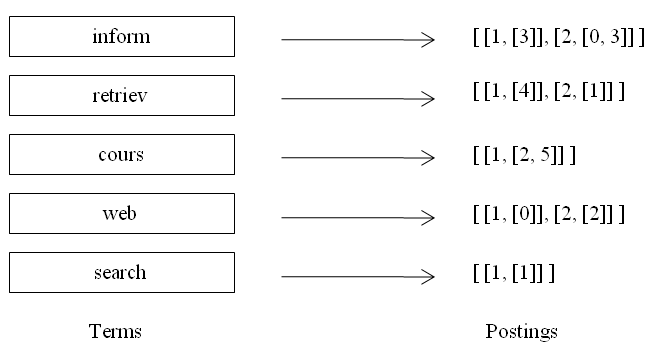
\includegraphics[width=0.5\textwidth]{images/inverted_index.png}
    \caption{Inverted Index}
    \label{fig:index}
\end{figure}
As we can see in the picture, there are mainly two parts of inverted index. The first part is a dictionary which contains the terms. Each key of the dictionary is a term. The dictionary can be implemented as hash or B-tree. The second part is the posting list of documents related to terms. The elements of the list are corresponding to the documents related to the terms, each of which contains the term frequency and the document id. Considering the size of index, we don't storage the contents of the documents. 

\subsubsection{Index Construction}
When the volume of data are large, it's not realistic to construct index of all data at one time. Further more, in practical environment of search engine, the data are generated in real time. Therefore, we use the Single-pass in-memeory indexing (SPIMI) algorithm. The pseudocode of SPIMI is:
\begin{figure}[H]
  \centering
    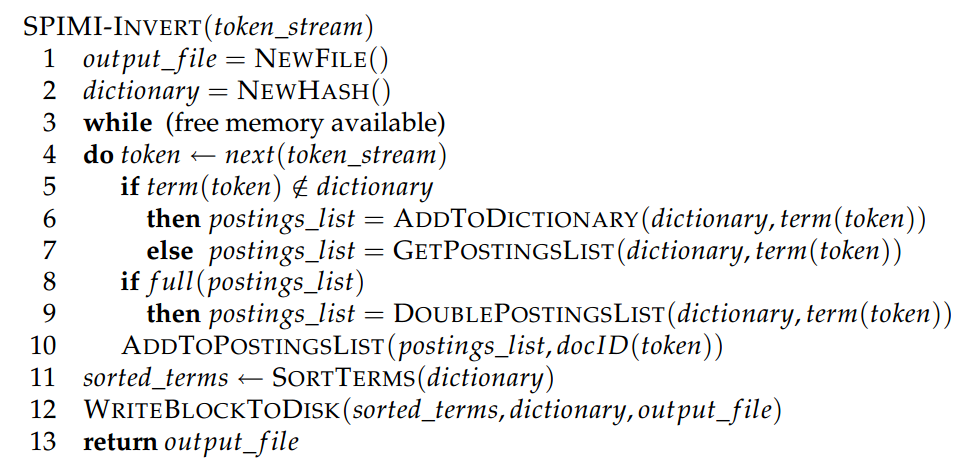
\includegraphics[width=0.5\textwidth]{images/SPIMI-algo.png}
    \caption{SPIMI Algorithm}
    \label{fig:spimi}
\end{figure}

\subsubsection{Regional Index}
To support advanced search of searching in questions or in answers or in specific tag, we support regional index. Specifically, we construct indexes for questions, answers and tags respectively. All indexes are stored in database to improve the reading and writing performance. The table of index is:
\begin{table}[H]
\centering
\begin{tabular}{cc}
\toprule
\multicolumn{2}{c}{\textbf{Table: index}} \\
\midrule
key                   & class             \\
\midrule
term (primary key)                    & TEXT               \\
df                   & INT               \\
docs                  & TEXT              \\
\bottomrule
\end{tabular}
\end{table}


\subsection{Search Model}
\label{subsec:search_engine}
All web pages are indexed and stored in the database after index procedure. Now we can build a search model for the search engine. We have many optional methods like vector distance, probability model, BM25 model and so on. The BM25\cite{robertson2009probabilistic} algorithm is very famous and has a good performance. We apply the BM25 model for searching.

\subsubsection{BM25 Search Model}
Okapi BM25(BM stands for Best Matching) algorithm is a ranking algorithm which can be used for search engines to estimate the relevance of documents to a given search query. The BM25 algorithm based on the probabilistic retrieval framework. It is a bag-of-words retrieval function that ranks a set of documents based on the query terms appearing in the documents, regardless of their proximity within the document. Our implementation of BM25 model based on the formula below:

\begin{equation*}
\begin{aligned}
BM25_{score}(Q, d) = \sum_{t\in Q}w(t,d)
\end{aligned}
\end{equation*}

\begin{equation*}
\begin{aligned}
w(t, d) = \frac{qtf}{k_3 + qtf} &\times \frac{k_1\times tf}{tf+k_1(1-b+b\times l_d / avg_l)} \\ 
&\times log_2\frac{N-df+0.5}{df+0.5}
\end{aligned}
\end{equation*}
In which, we have:
\begin{itemize}
    \item $qtf$: the word frequency of query
    \item $tf$: the word frequency of document
    \item $l_d$: length of document
    \item $avg_l$: average length of document
    \item $N$: number of documents
    \item $df$: the frequency of documents
    \item $b, k_1, k_3$: hyper-parameters
\end{itemize}

It is complicated but easy to understand. The first formula is an external formula. A query Q may contain multiple terms. For example, "install python" contains two terms "install" and "python". We need to calculate the contribution of “install” and “python” separately. The contribution scores of document $d$ are $w(t,d)$, and then adding them together is the score of the document $d$ for the query $Q$.

The second formula is to calculate the score of a term $t$ in document $d$, which consists of three parts. 

The first part is the score of the term $t$ in the query Q. For example, in the query "Chinese speaks Chinese", the term "China" appears twice, at this time qtf=2, indicating the document that the query hopes to find is more relevant with "China". In other words, the weight of ”China” should be greater, but in general, the query Q is very short and is unlikely to contain the same term, so this factor is a constant that we can ignore when we implement our system.

The second part is similar to the TF term in the TF-IDF model. That is to say, the more times a certain term $t$ appears in the document $d$, the more important $t$ is. But if the document becomes very long, the tf tends to be larger too. So we normalize the effect by using the length of the document divided by the average length, i.e. $l_d/avg_l$ . In this part, k1 and b are tun-able hyper parameters.

The third part is similar to the IDF item in the TF-IDF model. That is to say, although the stop words such as "a", "is", "are" appear many times in a document $d$, they have appeared in many documents, so the contribution of these words to $d$ is not high. Instead, words that appears very rare such as "diabetes" can distinguish between different documents, and the contribution of these words to the document should be higher.

Therefore, according to the BM25 formula, we can quickly calculate the scores of different documents $t$ on the query $Q$, and then give the results according to the ranking of the scores.
The pesduo code can be seen as the fllowing. The calculation procedure has been described in this part.
\begin{lstlisting}
import numpy as np
def BM25_alg(sentence, docs):
    seg_list = segmentation of sentence
    cleaned_dict = preprocess of seg_list
    BM25_scores = {}
    for term in cleaned_dict.keys():
        for doc in docs:
            calculate the BM25 score
    results = sort by BM25 score
    return results
\end{lstlisting}


\subsubsection{Query Preprocess}
We need to carry out preprocess of queries mainly because of two reasons. The first reason is that the user may enter a sentence with some meaningless terms or symbols. The second reason is that we must process the queries to find the search pattern of the query. For example, we use $[]$ to stands for field search. We must recognize it by preprocess of queries.

A little different with the preprocess of documents, we first recognize the patterns of the queries. If we find that the query is the pattern for field search, we can choose the corresponding search tool. And after the pattern recognization, we carry out a preprocess similar with the document part. We do tokenization, normalization and elimination.

Tokenization is to split the queries into pieces. We use the Natural Language Toolkit NLTK to tokenize, it first split the text into sentences by punctuation, and then uses regular expressions to tokenize sentences. 
Then we make normalization. A term is a normalized type that is included in the IR system's dictionary. Token normalization is the process of transforming tokens into a canonical form for better searching. For example, capital words are normalized. To normalize tokens, we first turn tokens in lower case form and eliminating numbers. Then we use Porter Stemmer to extract stems of tokens, which is called called stemming.
There are some common words which may occur in most documents, which should not consider when calculating relevance between query and documents. So before indexing, those stop words are filtered out.
Then we get the filter query and we can get it for BM25 ranking.


%\subsection{Search Backend}
%\label{subsec:search_backend}

\section{Results}
\label{sec:results}
In this section, we compare the performance of our search engine with Whoosh.

Whoosh is a library of classes and functions for indexing text and then searching the index. It allows users to develop custom search engines for their content. For example, if users were creating blogging software, users could use Whoosh to add a search function to allow users to search blog entries.

We choose a data set which size is 35.5M. It contains 4,999 questions and 6,055 answers. We build our search engine and Whoosh engine on the data set at the same time, and we compare the performance of the two search engines. 

First, we compare the two search engine's speed in building index. It takes 87 seconds to build index for our search engine, and for Whoosh, it takes 6 minutes. Our search engine is 4.13 times faster than Whoosh.

Then we test different queries to compare the results of the two search engine. We use five different queries: python, sklearn, print, index, hello world. And the number of searched results are listed below:

\begin{table}[H]
\centering
\caption{Number of searched results of our search engine and Whoosh}
\begin{tabular}{cccccc}
\toprule
      & python & sklearn & print & index & hello world \\
\midrule
our  & 360    & 6       & 745   & 469   & 177         \\
Whoosh & 425    & 7       & 771   & 575   & 70       \\  
\bottomrule
\end{tabular}
\end{table}

As we can see from the result, when we search only one word, our search engine returns a bit fewer results than Whoosh. When the query contains more than two words, our search engine returns more results than Whoosh. It is because our search engine also returns the search result of each word.

Here are the result of query "sklearn" of our search engine and Whoosh:\\
\begin{figure}[H]
  \centering
    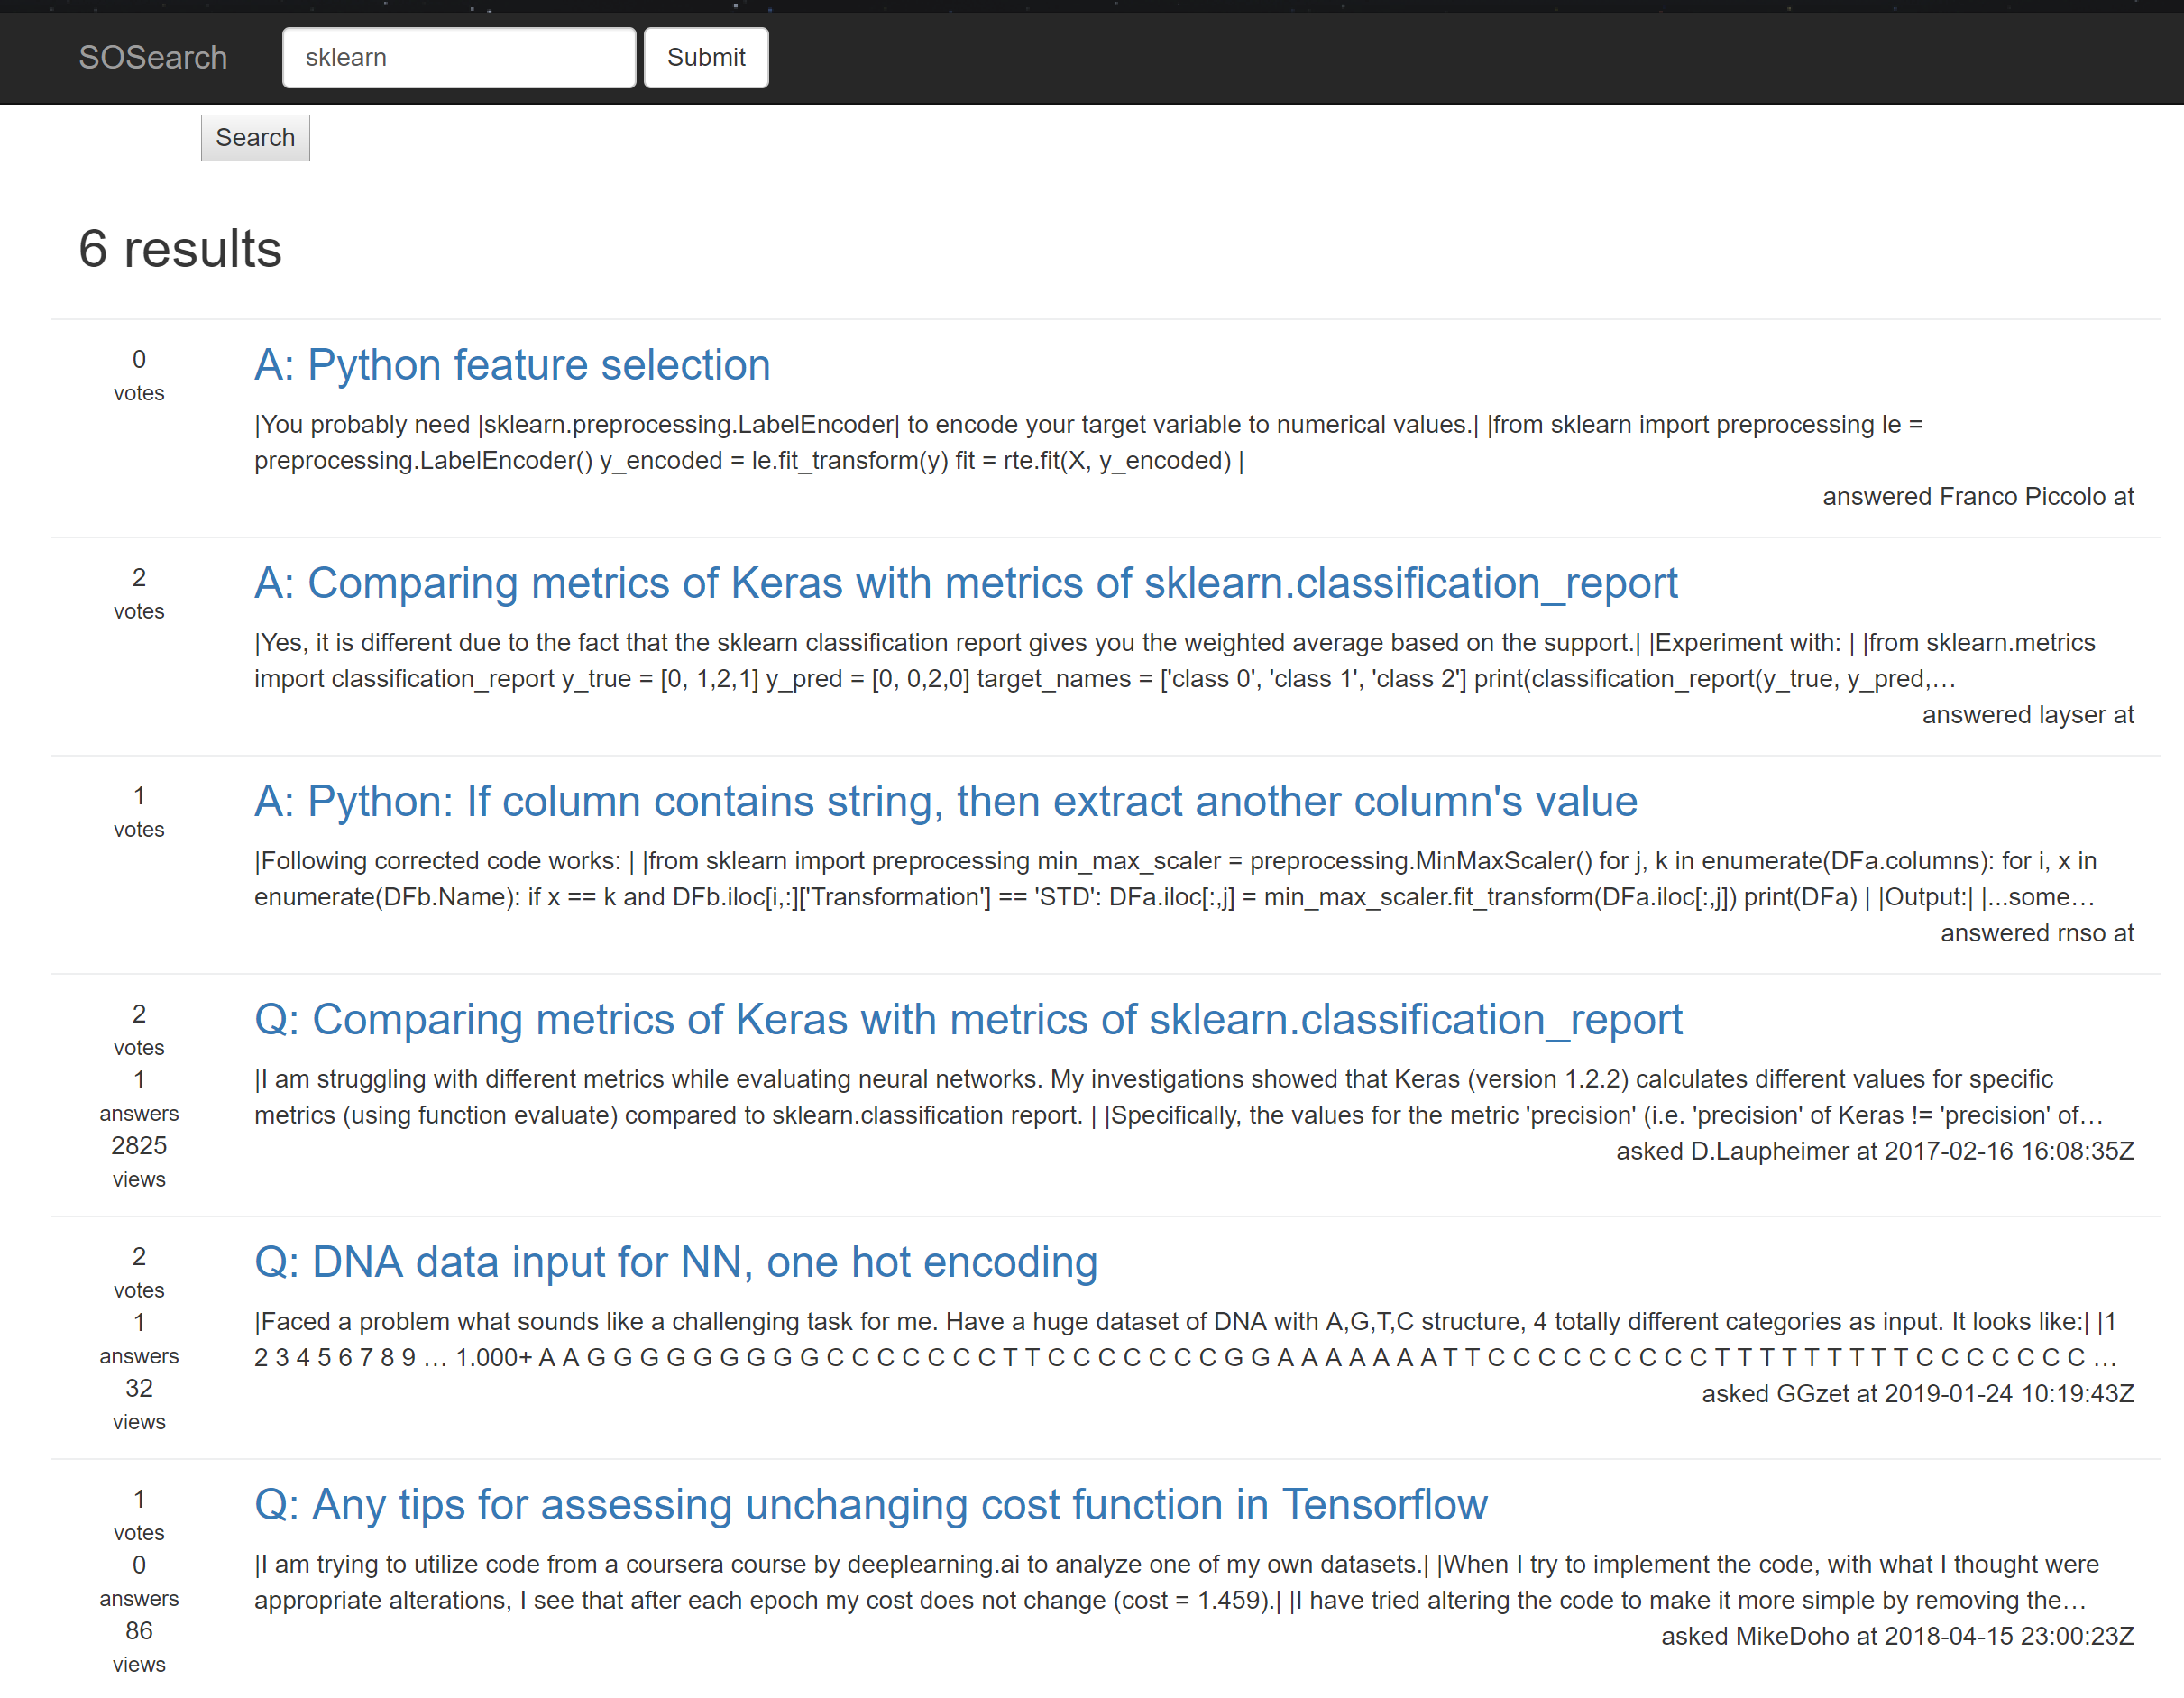
\includegraphics[width=0.5\textwidth]{images/testsklearn.png}
    \caption{Our model's searching results for "sklearn"}
\end{figure}

\begin{figure}[H]
  \centering
    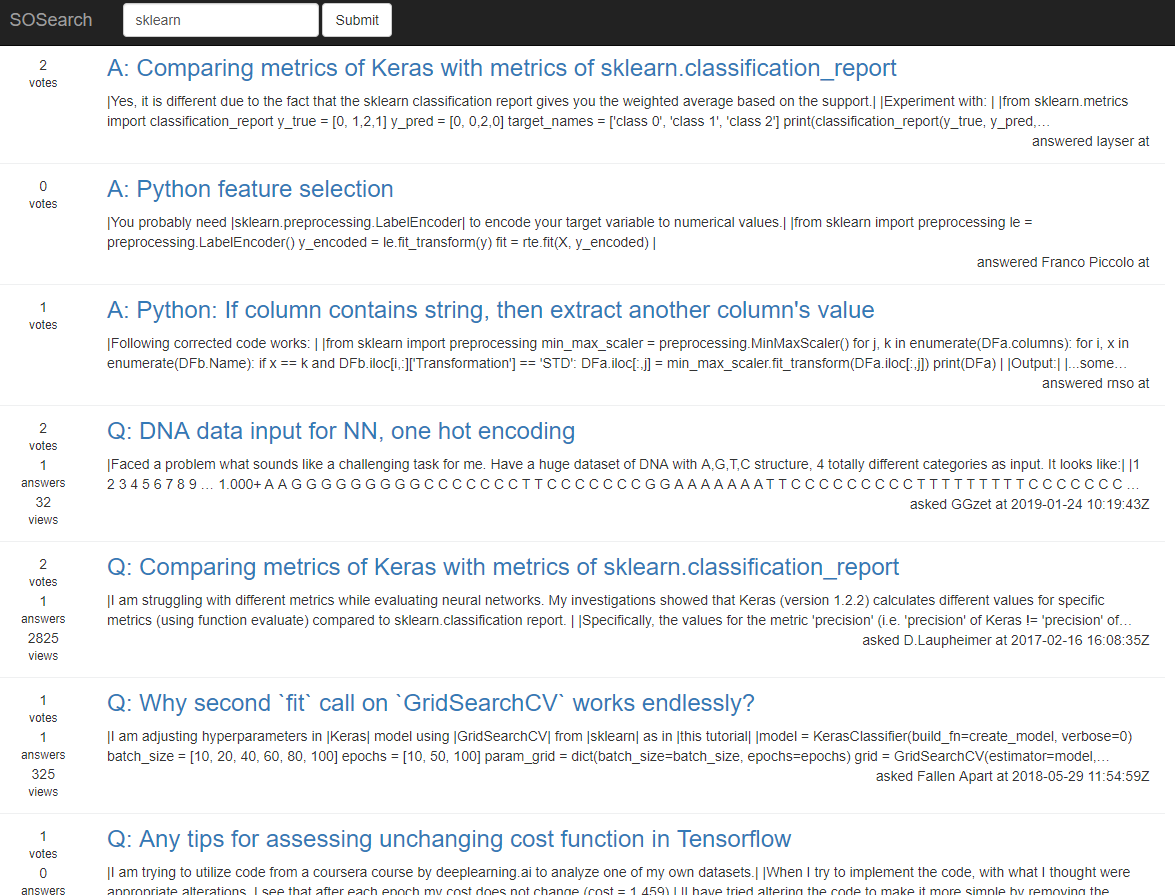
\includegraphics[width=0.5\textwidth]{images/whooshsklearn.png}
    \caption{Whoosh's searching results for "sklearn"}
\end{figure}

Comparing the two results, we can find that the two search engines return similar searching results.

\section{Conclusion}
\label{sec:conclusion}

In our report, we firstly introduce the design and implementation of our crawler. Then we introduce the database we store data and the web page of our search engine. The details of our search engine is introduced in Section ~\ref{sec:search_engine}. It contains the indexing part and the searching part. Finally, we compare the performance of our search engine with Whoosh.

% \begin{figure*}[!t]
%   \centering
%     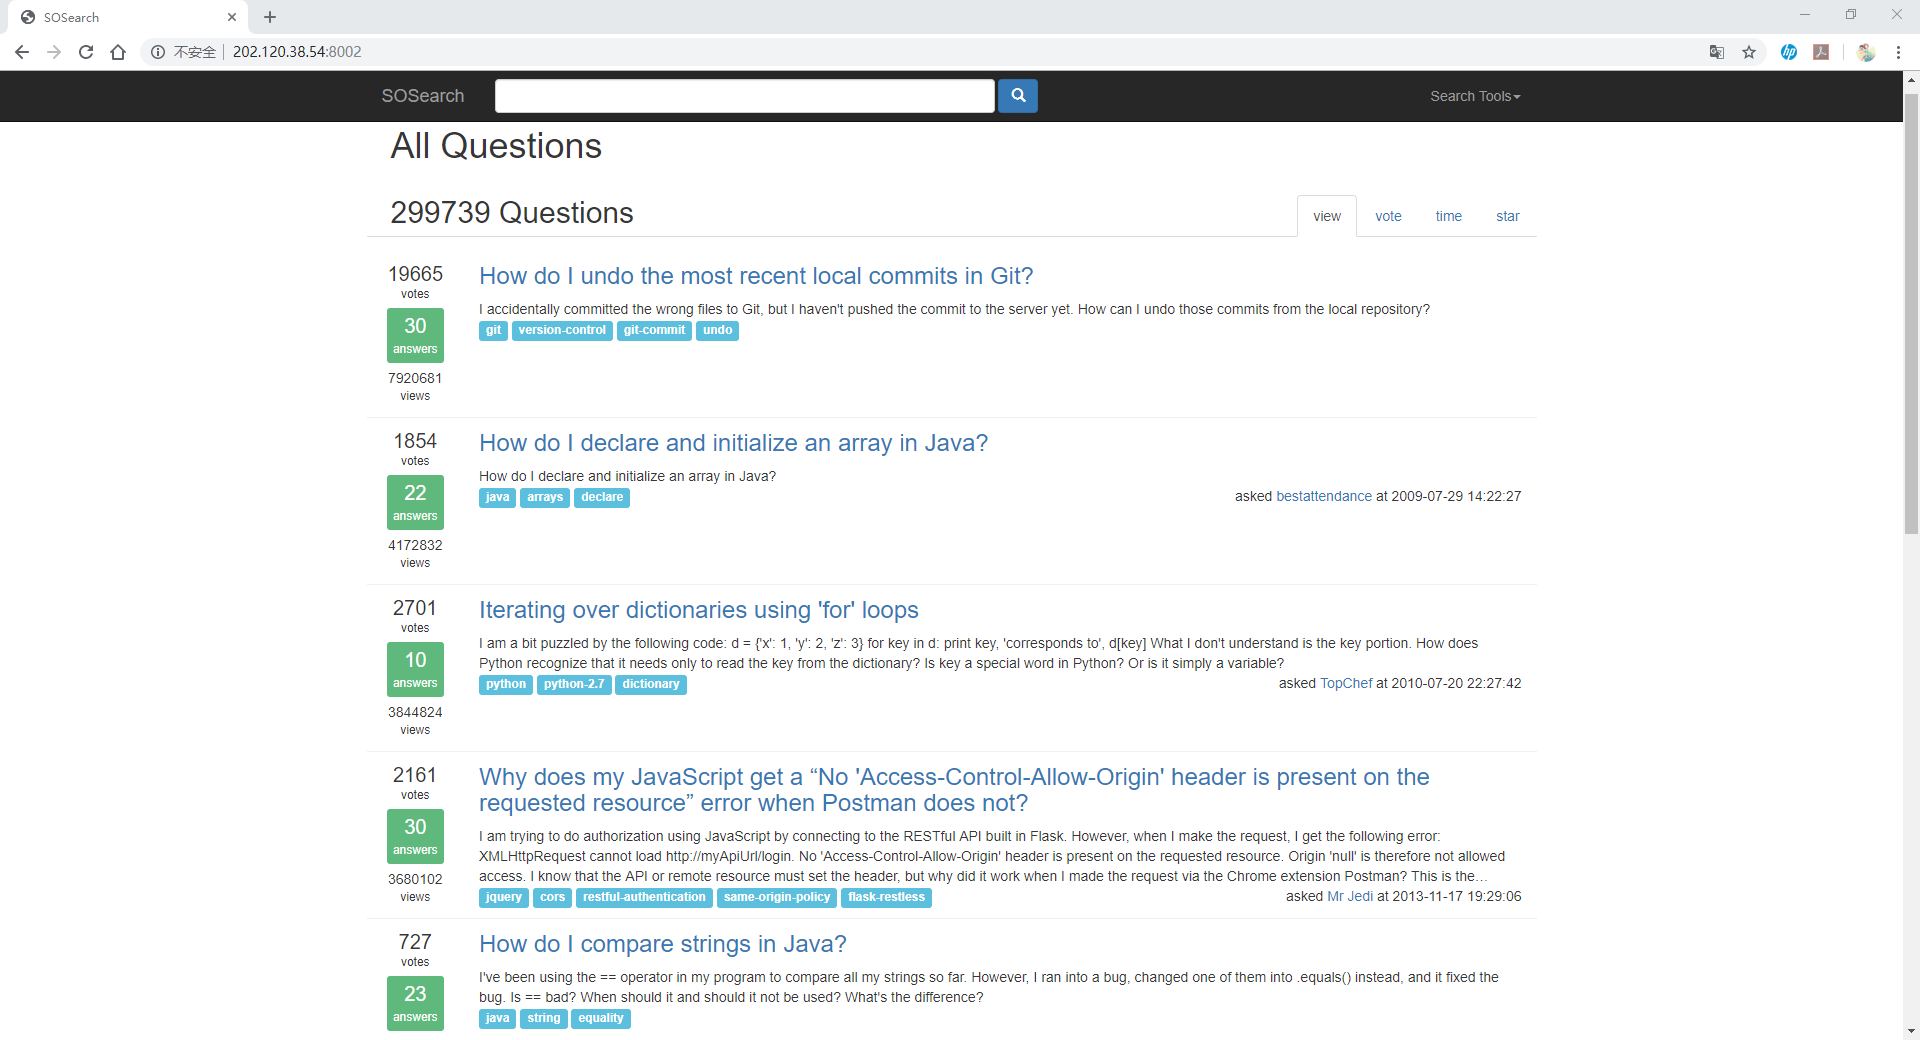
\includegraphics[width=1\textwidth]{images/large_index.png}
%     \caption{Index Page}
%     \label{fig:index}
% \end{figure*}

% \begin{figure*}[!t]
%   \centering
%     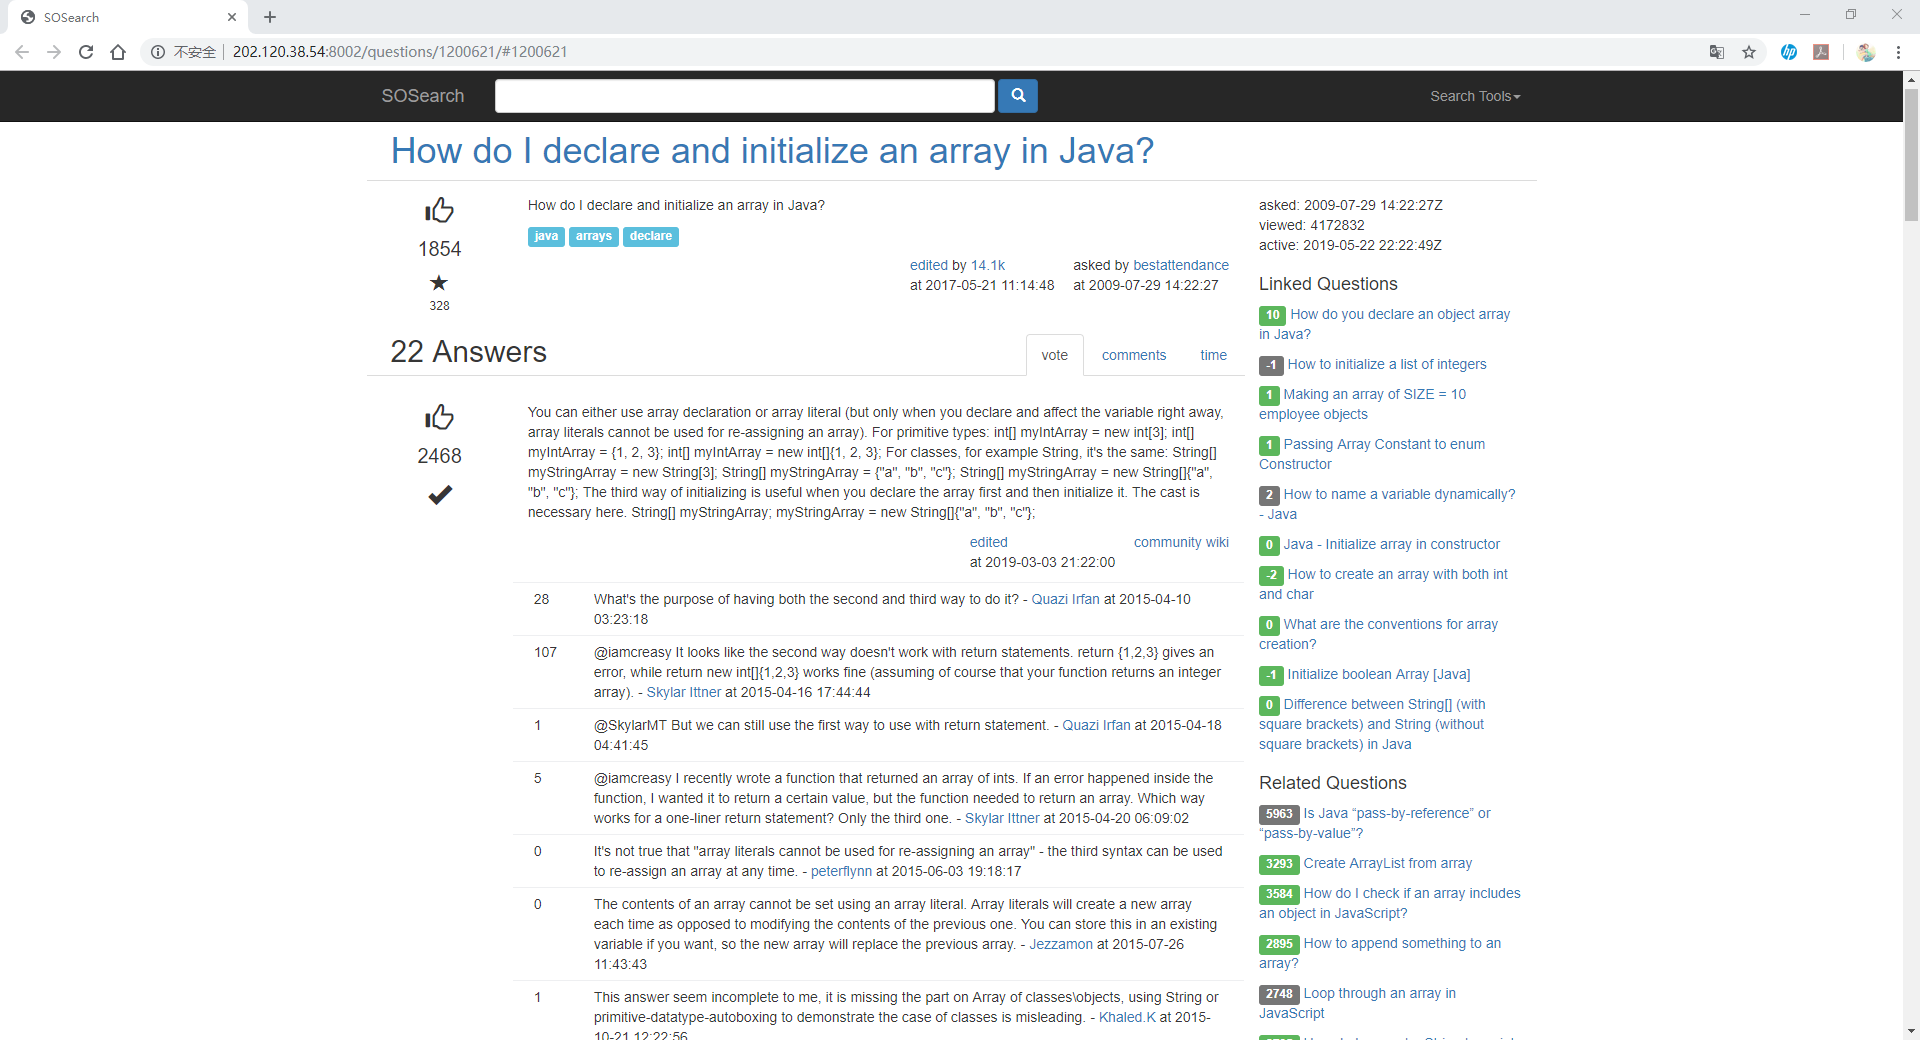
\includegraphics[width=1\textwidth]{images/large_detail.png}
%     \caption{Detail Page}
%     \label{fig:detail}
% \end{figure*}

% \begin{figure*}[!t]
%   \centering
%     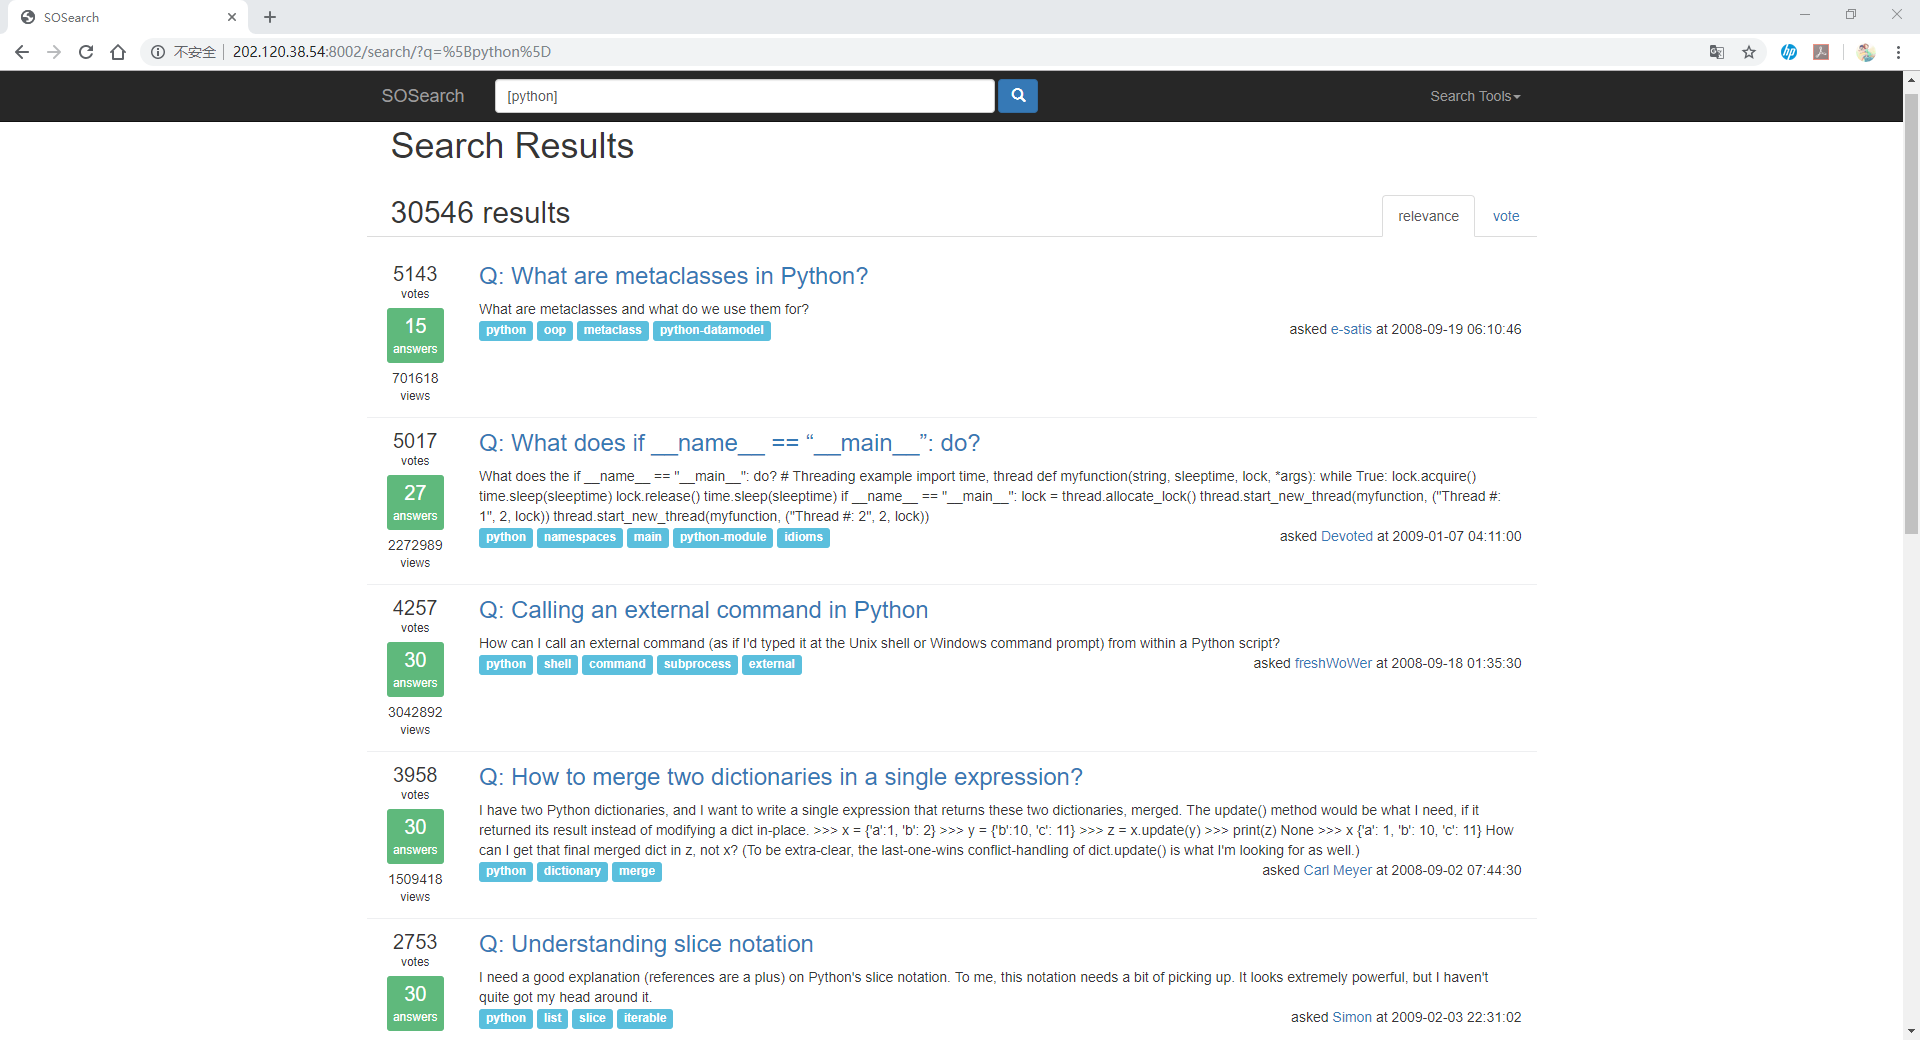
\includegraphics[width=1\textwidth]{images/large_search.png}
%     \caption{Search Page}
%     \label{fig:search}
% \end{figure*}



% use section* for acknowledgment
\ifCLASSOPTIONcompsoc
  % The Computer Society usually uses the plural form
  \section*{Acknowledgments}
\else
  % regular IEEE prefers the singular form
  \section*{Acknowledgment}
\fi


The authors would like to thank Prof. Kenny Q. Zhu and TA Flora Huang and Kelsey Huang for their instructions on this work.


% Can use something like this to put references on a page
% by themselves when using endfloat and the captionsoff option.
\ifCLASSOPTIONcaptionsoff
  \newpage
\fi



% trigger a \newpage just before the given reference
% number - used to balance the columns on the last page
% adjust value as needed - may need to be readjusted if
% the document is modified later
%\IEEEtriggeratref{8}
% The "triggered" command can be changed if desired:
%\IEEEtriggercmd{\enlargethispage{-5in}}

% references section

% can use a bibliography generated by BibTeX as a .bbl file
% BibTeX documentation can be easily obtained at:
% http://mirror.ctan.org/biblio/bibtex/contrib/doc/
% The IEEEtran BibTeX style support page is at:
% http://www.michaelshell.org/tex/ieeetran/bibtex/
%\bibliographystyle{IEEEtran}
% argument is your BibTeX string definitions and bibliography database(s)
%\bibliography{IEEEabrv,../bib/paper}
%
% <OR> manually copy in the resultant .bbl file
% set second argument of \begin to the number of references
% (used to reserve space for the reference number labels box)
\iffalse
\begin{thebibliography}{1}

\bibitem{IEEEhowto:kopka}
H.~Kopka and P.~W. Daly, \emph{A Guide to \LaTeX}, 3rd~ed.\hskip 1em plus
  0.5em minus 0.4em\relax Harlow, England: Addison-Wesley, 1999.

\end{thebibliography}
\fi

\bibliographystyle{IEEEtran}
\bibliography{reference}

% biography section
% 
% If you have an EPS/PDF photo (graphicx package needed) extra braces are
% needed around the contents of the optional argument to biography to prevent
% the LaTeX parser from getting confused when it sees the complicated
% \includegraphics command within an optional argument. (You could create
% your own custom macro containing the \includegraphics command to make things
% simpler here.)
%\begin{IEEEbiography}[{\includegraphics[width=1in,height=1.25in,clip,keepaspectratio]{mshell}}]{Michael Shell}
% or if you just want to reserve a space for a photo:


% You can push biographies down or up by placing
% a \vfill before or after them. The appropriate
% use of \vfill depends on what kind of text is
% on the last page and whether or not the columns
% are being equalized.

%\vfill

% Can be used to pull up biographies so that the bottom of the last one
% is flush with the other column.
%\enlargethispage{-5in}



% that's all folks
\end{document}


